\documentclass[aspectratio=169,11pt]{ctexbeamer}

\usetheme{Madrid}
\usecolortheme{default}
\setbeamertemplate{navigation symbols}{}
\setbeamertemplate{footline}[frame number]

\usepackage{amsmath,amssymb,bm,mathtools}
\usepackage{booktabs}
\usepackage{graphicx}
\usepackage{tikz}
\usetikzlibrary{arrows.meta,positioning,calc}

\definecolor{idealblue}{RGB}{42,91,160}
\definecolor{errororange}{RGB}{213,111,34}
\definecolor{urcteal}{RGB}{19,133,123}
\definecolor{softgray}{RGB}{105,105,105}

\tikzset{
  urcbox/.style={
    draw,
    rounded corners=2pt,
    align=center,
    minimum height=8mm,
    inner sep=4pt
  },
  urcarrow/.style={-{Latex[length=2mm]},thick}
}

\newcommand{\Tr}{\operatorname{Tr}}
\newcommand{\Vbar}{\overline V_0}
\newcommand{\Mtilde}{\widetilde M_0}
\newcommand{\source}[1]{%
  \par\vspace{0.4mm}{\tiny\color{softgray}Source: #1}%
}
\newcommand{\explain}[1]{%
  \par\vspace{0.4mm}{\footnotesize #1}\par\vspace{0.4mm}%
}
\newcommand{\insight}[1]{%
  \par\vspace{0.4mm}{\footnotesize\color{idealblue}#1}\par\vspace{0.4mm}%
}

\title[Universally Robust Quantum Control]
{Universally Robust Quantum Control}
\subtitle{从 fidelity susceptibility 到 unitary 1-design}
\author{Noise-Tolerant Quantum Control Optimization}
\date{\today}

\begin{document}

\begin{frame}
  \titlepage
  \source{Poggi et al., Phys. Rev. Lett. 132, 193801 (2024);
  arXiv:2309.14437v2}
\end{frame}

\begin{frame}{未知系统误差}
  \explain{设受控系统的 Hilbert 空间维数为 \(d\)，理想控制由
  \(H_0(t)\) 产生；实际 Hamiltonian 含有一个未知的静态相干误差。}
  \[
    \textcolor{idealblue}{H_0(t)}
    \quad\longrightarrow\quad
    H_\lambda(t)
    =\textcolor{idealblue}{H_0(t)}
    +\textcolor{errororange}{\lambda V},
  \]
  \[
    |\lambda|\ll1,
    \qquad V=V^\dagger,
    \qquad
    U_\lambda(t_f,0)
    =\mathcal T\exp\!\left[
      -\frac{i}{\hbar}\int_0^{t_f}H_\lambda(t)\,dt
    \right].
  \]

  \explain{
    \(\lambda\) 是无量纲小参数，\(V=V^\dagger\) 给出误差方向；
    当前框架讨论 systematic Hamiltonian error，不包含 decay 或一般
    Lindblad dissipator。
  }
  \insight{控制目标：实现 target gate，同时压低 fidelity 对允许误差方向的响应。}
  \[
    \boxed{
    U_0(t_f,0)=U_{\mathrm{target}},
    \qquad
    1-F(\lambda)=O(\lambda^2)
    }
  \]
\end{frame}

\begin{frame}{已知 \(V\) 与未知 \(V\)}
  \explain{
    物理上用 \(\mathfrak{su}(d)\) 表示 \(d\times d\) traceless
    Hermitian generators；与数学中 anti-Hermitian convention 相差因子 \(i\)。
    Identity 分量只产生 global phase。
  }
  \begin{center}
    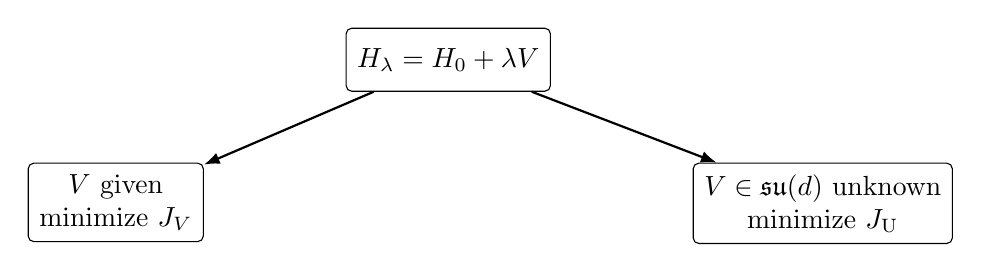
\begin{tikzpicture}[node distance=9mm and 18mm]
      \node[urcbox] (h) {\(H_\lambda=H_0+\lambda V\)};
      \node[urcbox,below left=of h] (known)
        {\(V\) given\\minimize \(J_V\)};
      \node[urcbox,below right=of h] (unknown)
        {\(V\in\mathfrak{su}(d)\) unknown\\minimize \(J_{\mathrm U}\)};
      \draw[urcarrow] (h) -- (known);
      \draw[urcarrow] (h) -- (unknown);
    \end{tikzpicture}
  \end{center}

  \insight{已知 \(V\) 时只压低一个方向；未知 \(V\) 时，同一条
  \(U_0(t)\) 必须对整个 traceless operator space 都不敏感。}
\end{frame}

\begin{frame}{纯态 fidelity：二阶项}
  \small
  \explain{先固定纯初态
  \(\sigma=|\psi\rangle\langle\psi|\)，比较理想末态
  \(\rho_0\) 与含误差末态 \(\rho_\lambda\)。}
  \[
    \rho_\lambda=U_\lambda\sigma U_\lambda^\dagger,
    \qquad
    F(\lambda)=\Tr(\rho_\lambda\rho_0),
    \qquad
    \rho_\lambda^2=\rho_\lambda.
  \]
  \explain{点记号表示在 \(\lambda=0\) 处求导：
  \(\dot\rho_0\equiv
  (\partial_\lambda\rho_\lambda)_{\lambda=0}\)。}
  \[
    \partial_\lambda(\rho_\lambda^2)=\partial_\lambda\rho_\lambda
    \quad\Longrightarrow\quad
    F'(0)=0.
  \]
  \explain{Projector 的 idempotency 与 trace normalization 使
  fidelity 在理想点没有一阶变化，leading error 因而从二阶开始。}
  \[
    \partial_\lambda^2(\rho_\lambda^2)
    =\partial_\lambda^2\rho_\lambda
    \quad\Longrightarrow\quad
    F''(0)=-2\Tr(\rho_0\dot\rho_0^2).
  \]
  \[
    \boxed{
    F(\lambda)=1-\chi_S\lambda^2+O(\lambda^3),
    \qquad
    \chi_S\equiv\Tr(\rho_0\dot\rho_0^2)
    }
  \]
\end{frame}

\begin{frame}{参数响应生成元}
  \small
  \explain{积分变量 \(s\in[0,t_f]\) 枚举持续存在的误差在整个演化期间的贡献；
  它不是误差在某个时刻才突然插入的随机事件。}
  \[
    \partial_\lambda U_\lambda(t_f,0)
    =-\frac{i}{\hbar}\int_0^{t_f}
    U_\lambda(t_f,s)VU_\lambda(s,0)\,ds .
  \]
  \explain{利用 propagator 的 composition property，把每个 \(s\) 时刻的响应
  统一搬运到末时刻 \(t_f\)。}
  \[
    U_\lambda(s,0)
    =U_\lambda^\dagger(t_f,s)U_\lambda(t_f,0)
  \]
  \[
    \Longrightarrow\qquad
    \partial_\lambda U_\lambda(t_f,0)
    =-iG_\lambda U_\lambda(t_f,0),
  \]
  \explain{
    \(G_\lambda=G_\lambda^\dagger\) 是参数变化在末态 unitary 上诱导的
    local generator；它同时生成末态 density operator 的变化。
  }
  \[
    G_\lambda=
    \frac1\hbar\int_0^{t_f}
    U_\lambda(t_f,s)VU_\lambda^\dagger(t_f,s)\,ds,
    \qquad
    \boxed{\partial_\lambda\rho_\lambda
    =-i[G_\lambda,\rho_\lambda]} .
  \]
\end{frame}

\begin{frame}{Interaction-picture 时间平均}
  \small
  \explain{Interaction picture 剥离已知的理想控制，只保留误差
  \(V\) 被理想轨迹旋转后的累积效果。}
  \[
    \Vbar\equiv\frac1{t_f}\int_0^{t_f}
    U_0^\dagger(s,0)VU_0(s,0)\,ds .
  \]
  \[
    G_0
    =U_0(t_f,0)
    \left(\frac{t_f}{\hbar}\Vbar\right)
    U_0^\dagger(t_f,0).
  \]
  \[
    \boxed{
    \chi_S
    =\frac{t_f^2}{\hbar^2}
    (\Delta_\sigma\Vbar)^2
    }
  \]
  \explain{
    \(\Delta_\sigma\Vbar\) 不是误差参数的变化量，而是算符
    \(\Vbar\) 在初态 \(\sigma\) 上的 standard deviation：
  }
  \[
    (\Delta_\sigma\Vbar)^2
    =\Tr(\sigma\Vbar^2)-[\Tr(\sigma\Vbar)]^2 .
  \]
  \insight{只有不能被该状态视为 global phase 的平均误差分量才降低 state fidelity。}
\end{frame}

\begin{frame}{QFI：只需要这一条联系}
  \small
  \explain{Quantum Fisher information (QFI) 衡量量子态对参数
  \(\lambda\) 的局部可区分性；\(L_\lambda=L_\lambda^\dagger\) 是
  symmetric logarithmic derivative (SLD)。}
  \[
    \partial_\lambda\rho_\lambda
    =\frac12(\rho_\lambda L_\lambda+L_\lambda\rho_\lambda),
    \qquad
    F_Q=\Tr(\rho_\lambda L_\lambda^2).
  \]
  \explain{对纯态，在其 support 上可取
  \(L_\lambda=2\partial_\lambda\rho_\lambda\)，因此 QFI 是状态沿参数方向
  运动速度的平方。}
  \[
    \rho_\lambda^2=\rho_\lambda
    \quad\Longrightarrow\quad
    L_\lambda=2\partial_\lambda\rho_\lambda
  \]
  \[
    \Longrightarrow\qquad
    F_Q
    =4\Tr\!\left[
      \rho_\lambda(\partial_\lambda\rho_\lambda)^2
    \right].
  \]
  \[
    \boxed{
      F_Q\big|_{\lambda=0}=4\chi_S
    }
  \]
  \insight{这里 \(F_Q=4\chi_S\) 在 fidelity 的展开点 \(\lambda=0\) 使用。}
\end{frame}

\begin{frame}{Gate fidelity 与 Dyson 展开}
  \small
  \explain{State fidelity 固定一个输入态；gate fidelity 直接比较两个
  \(d\times d\) unitary 在整个 Hilbert 空间上的重合。}
  \[
    F_U(\lambda)=\frac1{d^2}
    \left|\Tr(U_0^\dagger U_\lambda)\right|^2,
    \qquad
    U_\lambda(t_f,0)=U_0(t_f,0)U_I(t_f,0).
  \]
  \explain{分母 \(d^2\) 来自 \(\Tr\mathbb I=d\)，保证
  \(U_\lambda=U_0\) 时 \(F_U=1\)；提出理想演化后，\(U_I\) 只包含误差。}
  \[
    U_I
    =\mathcal T\exp\!\left[
      -\frac{i\lambda}{\hbar}
      \int_0^{t_f}V_I(s)\,ds
    \right],
    \quad
    V_I(s)=U_0^\dagger(s,0)VU_0(s,0).
  \]
  \explain{为提取 leading infidelity，只需将 time-ordered exponential
  展开到 \(\lambda^2\)。}
  \[
    U_I=\mathbb I-\frac{i\lambda}{\hbar}A
    -\frac{\lambda^2}{\hbar^2}B+O(\lambda^3),
    \qquad
    A=\int_0^{t_f}V_I(s)\,ds=t_f\Vbar .
  \]
\end{frame}

\begin{frame}{一般 gate susceptibility}
  \small
  \[
    F_U(\lambda)
    =1-\frac{\lambda^2t_f^2}{\hbar^2d}
    \left[
      \Tr(\Vbar^2)
      -\frac{|\Tr\Vbar|^2}{d}
    \right]
    +O(\lambda^3).
  \]
  \explain{方括号是 \(\Vbar\) 去除 identity 分量后的平方大小；
  identity 只给 unitary 增加不可观测的 global phase。}
  \[
    \Vbar^{\mathrm{tl}}
    =\Vbar-\frac{\Tr(\Vbar)}d\mathbb I,
  \]
  \explain{上标 \(\mathrm{tl}\) 表示 traceless part，而不是新的误差算符。}
  \[
    \boxed{
    \chi_U=\frac{t_f^2}{\hbar^2d}
    \Tr\!\left[
      \left(\Vbar^{\mathrm{tl}}\right)^2
    \right]
    }.
  \]
  \insight{因此 \(\chi_U\) 衡量整扇门的一阶 error generator 在物理相关方向上的大小。}
\end{frame}

\begin{frame}{论文采用 traceless \(V\)}
  \small
  \explain{任意 Hermitian error 都可唯一分成 identity 与 traceless 两部分；
  论文直接在后者上讨论 robustness。}
  \[
    \Tr V=0
    \quad\Longrightarrow\quad
    \Tr\Vbar=0
    \quad\Longrightarrow\quad
    \Vbar^{\mathrm{tl}}=\Vbar .
  \]
  \[
    \boxed{
    \chi_U
    =\frac{t_f^2}{\hbar^2d}
    \Tr(\Vbar^2)
    }
  \]
  \[
    \Vbar=0
    \quad\Longleftrightarrow\quad
    \text{first-order error generator is cancelled}.
  \]
  \insight{此时 Dyson/Magnus 展开的一阶生成元消失，因而 gate infidelity 的
  \(\lambda^2\) 系数为零。}
\end{frame}

\begin{frame}{Operator Hilbert space}
  \small
  \explain{为同时处理所有误差方向，把 \(d\times d\) 算符视为
  \(d^2\) 维 operator Hilbert space 中的向量；圆括号 ket 用来和物理态区分。}
  \[
    A=\sum_{ij}A_{ij}|i\rangle\langle j|
    \quad\longmapsto\quad
    |A)=\sum_{ij}A_{ij}|i\rangle\otimes|j\rangle .
  \]
  \[
    (A|B)=\Tr(A^\dagger B),
    \qquad
    \dim(\mathcal H\otimes\mathcal H^*)=d^2 .
  \]
  \explain{Hilbert--Schmidt inner product 把算符的平方大小变成普通向量范数。}
  \explain{Vectorization 的关键作用，是把共轭变换
  \(V\mapsto U^\dagger VU\) 写成一个矩阵对 \(|V)\) 的线性作用：}
  \[
  \begin{aligned}
    |U^\dagger VU)
    &=(U^\dagger\otimes U^T)|V)\\
    &=(U\otimes U^*)^\dagger|V).
  \end{aligned}
  \]
\end{frame}

\begin{frame}{共轭平均写成超算符}
  \small
  \explain{
    \(M_0\) 完全由理想控制轨迹 \(U_0(s)\) 决定：输入任意误差方向
    \(|V)\)，输出该方向的 interaction-picture 时间平均 \(|\Vbar)\)。
  }
  \[
    |\Vbar)
    =\frac1{t_f}\int_0^{t_f}
    [U_0(s)\otimes U_0(s)^*]^\dagger|V)\,ds .
  \]
  \[
    \boxed{
    M_0\equiv\frac1{t_f}\int_0^{t_f}
    [U_0(s)\otimes U_0(s)^*]^\dagger ds
    },
    \qquad
    \boxed{|\Vbar)=M_0|V)} .
  \]
  \begin{center}
    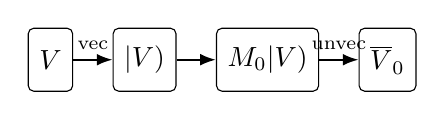
\begin{tikzpicture}[node distance=5mm]
      \node[urcbox] (v) {\(V\)};
      \node[urcbox,right=of v] (vecv) {\(|V)\)};
      \node[urcbox,right=of vecv] (mv) {\(M_0|V)\)};
      \node[urcbox,right=of mv] (vbar) {\(\Vbar\)};
      \draw[urcarrow] (v) --
        node[above,font=\scriptsize]{vec} (vecv);
      \draw[urcarrow] (vecv) -- (mv);
      \draw[urcarrow] (mv) --
        node[above,font=\scriptsize]{unvec} (vbar);
    \end{tikzpicture}
  \end{center}
  \insight{Universal optimization 不必预先知道实际 \(V\)，而是直接压低
  整个线性映射 \(M_0\) 在 traceless 子空间上的作用。}
\end{frame}

\begin{frame}{已知误差是一个二次型}
  \small
  \explain{固定一个已知 \(V\) 后，susceptibility 就是输出
  \(|\Vbar)\) 的 Hilbert--Schmidt norm squared。}
  \[
    |\Vbar)=M_0|V)
    \quad\Longrightarrow\quad
    (\Vbar|\Vbar)
    =(V|M_0^\dagger M_0|V).
  \]
  \[
    \boxed{
    \chi_U(V)
    =\frac{t_f^2}{\hbar^2d}
    (V|M_0^\dagger M_0|V)
    }.
  \]
  \explain{只有反向量化回算符后才写 trace；vectorized quantity 本身使用
  圆括号内积。}
  \[
    (\Vbar|\Vbar)
    =\Tr(\Vbar^\dagger\Vbar)
    =\Tr(\Vbar^2),
  \]
  \[
    V=V^\dagger
    \quad\Longrightarrow\quad
    \Vbar=\Vbar^\dagger .
  \]
\end{frame}

\begin{frame}{去掉 identity 方向}
  \small
  \explain{共轭演化永远保持 identity，因此 \(M_0\) 不可能在整个
  \(d^2\) 维 operator space 上趋于零。}
  \[
    U_0^\dagger\mathbb I U_0=\mathbb I
    \quad\Longrightarrow\quad
    M_0|\mathbb I)=|\mathbb I).
  \]
  \[
    \mathbb P_0
    =\frac{|\mathbb I)(\mathbb I|}{d},
    \qquad
    \mathbb P_0|A)
    =\frac{\Tr A}{d}|\mathbb I).
  \]
  \[
    \boxed{
      \Mtilde=M_0(\mathbb I-\mathbb P_0)
    }
  \]
  \explain{
    \(\mathbb I-\mathbb P_0\) 先把输入限制到 traceless subspace；
    \(\Mtilde\) 才是 universal robustness 真正需要压低的响应。
  }
  \[
    (\mathbb I-\mathbb P_0)|A)
    =\left|A-\frac{\Tr A}{d}\mathbb I\right).
  \]
\end{frame}

\begin{frame}{三个优化目标}
  \small
  \explain{
    \(J_0\) 保证 target gate；\(J_V\) 压低一个已知误差方向；
    \(J_{\mathrm U}\) 汇总所有 traceless 正交方向。
  }
  \[
    J_0
    =1-\frac1{d^2}
    |\Tr(U_{\mathrm{target}}^\dagger U_0)|^2 .
  \]
  \[
    J_V
    =\frac1d(\Vbar|\Vbar)
    =\frac1d\Tr(\Vbar^2),
    \qquad
    J_{\mathrm U}
    =\frac1d\|\Mtilde\|_F^2 .
  \]
  \[
    \|X\|_F^2\equiv\Tr(X^\dagger X).
  \]
  \explain{对任意 traceless 正交基 \(\{|B_a)\}\)，
  \(\|\Mtilde\|_F^2=\sum_a\|\Mtilde|B_a)\|^2\)，所以
  \(J_{\mathrm U}\) 不偏向某个具体 \(V\)。}
  \[
  \begin{array}{c@{\qquad}c@{\qquad}c}
    J_0 & J_V & J_{\mathrm U}\\[1mm]
    \text{target only}
    & \text{known }V
    & \text{all traceless }V
  \end{array}
  \]
\end{frame}

\begin{frame}{Haar twirling 与 unitary 1-design}
  \small
  \explain{Haar measure \(\mu_{\mathrm H}\) 是 unitary group 上左右不变的
  均匀概率测度；twirling 对所有共轭方向作均匀平均。}
  \[
    \int_{\mathrm U(d)}
    U^\dagger A U\,d\mu_{\mathrm H}(U)
    =\frac{\Tr A}{d}\mathbb I .
  \]
  \explain{若带权集合 \(\{(p_k,U_k)\}\) 对任意算符 \(A\) 复制这一
  first moment，就称为 unitary 1-design。}
  \[
    \boxed{
    \sum_kp_kU_k^\dagger A U_k
    =\frac{\Tr A}{d}\mathbb I
    \quad\forall A
    }
  \]
  \[
    \Longleftrightarrow\qquad
    \boxed{
    \sum_kp_k(U_k\otimes U_k^*)^\dagger
    =\mathbb P_0
    }.
  \]
  \insight{这里仅匹配一次 \(U\) 和一次 \(U^*\)，不要求成为更强的 2-design。}
\end{frame}

\begin{frame}{1-design \(\Longrightarrow\) universal robustness}
  \small
  \explain{把连续控制轨迹按驻留时间离散化后，\(p_k\) 是轨迹停留在
  \(U_k\) 附近的时间权重。}
  \[
    M_0
    \simeq\sum_kp_k(U_k\otimes U_k^*)^\dagger .
  \]
  \[
    M_0=\mathbb P_0
    \quad\Longrightarrow\quad
    \Mtilde
    =\mathbb P_0(\mathbb I-\mathbb P_0)=0 .
  \]
  \explain{1-design 只保留 identity 分量，因此与 identity 正交的每个
  traceless \(|V)\) 都被映到零。}
  \[
    \boxed{
      M_0|V)=0
      \quad\forall\,V:\Tr V=0
    }
  \]
  \[
    \textcolor{urcteal}{
      \text{one unitary path}
      \quad\Longleftrightarrow\quad
      \text{all traceless error directions}
    }.
  \]
\end{frame}

\begin{frame}{单量子比特 Pauli 1-design}
  \small
  \explain{
    \(\sigma_x,\sigma_y,\sigma_z\) 是 Pauli operators；任意单量子比特算符
    都由 identity 部分 \(a_0\mathbb I\) 与 Bloch-vector 部分
    \(\bm a\cdot\bm\sigma\) 组成。
  }
  \[
    \mathcal E_{\mathrm P}
    =\{\mathbb I,\sigma_x,\sigma_y,\sigma_z\},
    \qquad p_k=\frac14 .
  \]
  \[
    A=a_0\mathbb I+\bm a\cdot\bm\sigma
  \]
  \[
    \Longrightarrow\qquad
    \frac14\sum_{P\in\mathcal E_{\mathrm P}}
    P^\dagger A P
    =a_0\mathbb I
    =\frac{\Tr A}{2}\mathbb I .
  \]
  \[
    \boxed{
      \bm a\cdot\bm\sigma
      \quad\xrightarrow{\text{Pauli twirl}}\quad0
    }
  \]
  \insight{四次 Pauli conjugation 使三个 Bloch 分量正负成对抵消，只留下
  \(a_0\mathbb I=(\Tr A/2)\mathbb I\)。}
\end{frame}

\begin{frame}{单量子比特控制模型}
  \small
  \[
    H_0(t)=\Omega\!\left[
      \cos\phi(t)\sigma_x+\sin\phi(t)\sigma_y
    \right],
    \qquad
    U_{\mathrm{target}}=e^{-i\pi\sigma_z/2}.
  \]
  \explain{
    \(\Omega\) 是固定驱动幅度，分段常数 \(\phi_k\) 是 GRAPE 优化变量；
    target 是绕 \(z\) 轴的 \(\pi\) rotation（相差一个 global phase）。
  }
  \[
    \phi(t)=\phi_k,
    \qquad
    t\in[(k-1)\Delta t,k\Delta t).
  \]

  \explain{\(t_{\mathrm{MCT}}\) 表示达到相应 objective 所需的
  minimum control time。}
  \[
  \begin{array}{c|ccc}
    \text{objective}
    & J_0
    & J_0+J_{V=\sigma_z}
    & J_0+J_{\mathrm U}\\
    \midrule
    t_{\mathrm{MCT}}
    & 2\pi/\Omega
    & 4\pi/\Omega
    & 5\pi/\Omega
  \end{array}
  \]
  \insight{从 target-only 到 known-error 再到 universal robustness，
  受约束的误差方向增多，因此需要更长轨迹完成近似 1-design。}
\end{frame}

\begin{frame}{单量子比特：已知方向与未知方向}
  \centering
  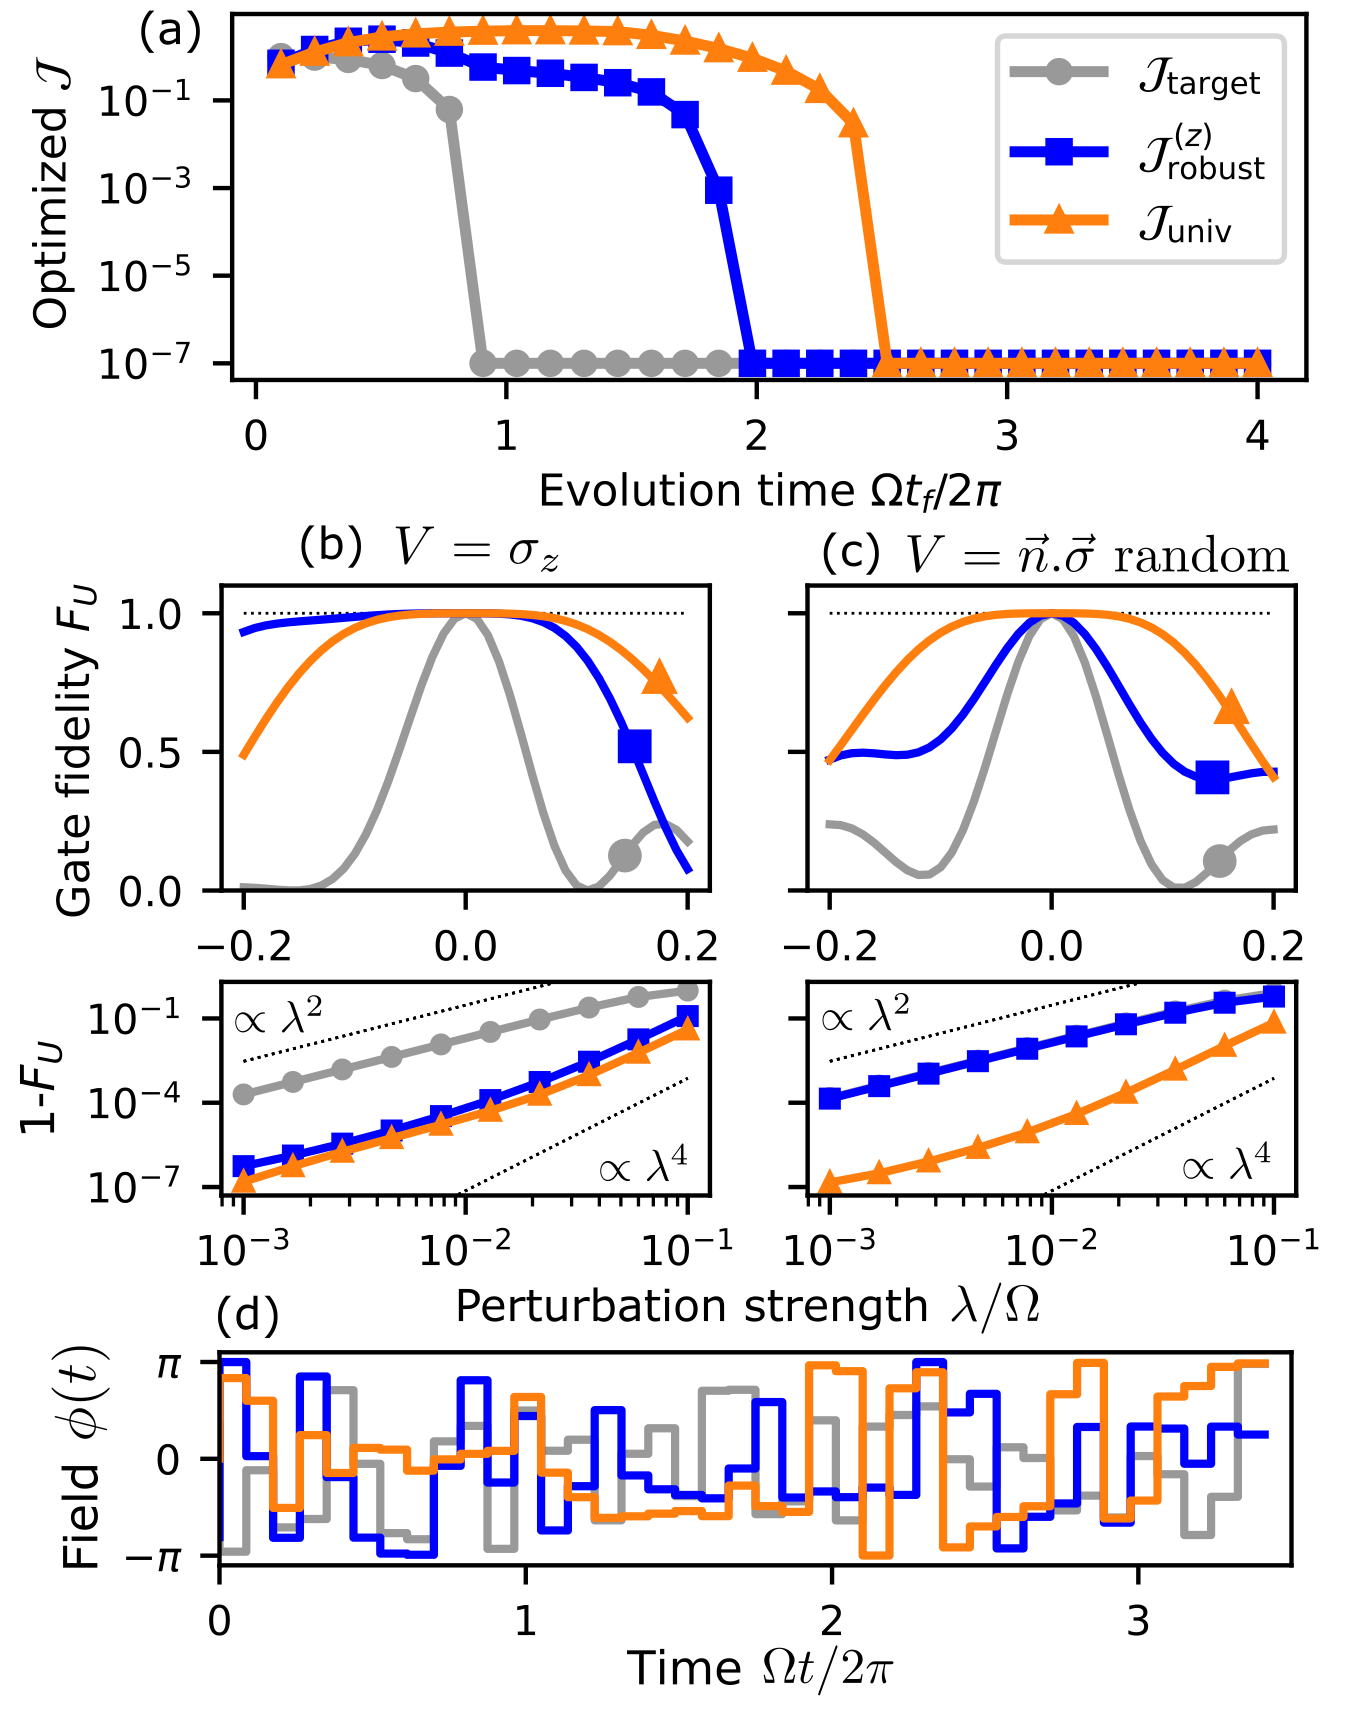
\includegraphics[
    width=0.92\textwidth,
    height=0.67\textheight,
    keepaspectratio,
    trim=0 38 0 95,
    clip
  ]{figures/poggi2024_fig1.png}

  \vspace{-1.5mm}
  {\scriptsize
    灰/蓝/橙分别表示 target-only、known-error robust 与 URC。\par
    左列 \(V=\sigma_z\) 时蓝、橙均有 \(1-F_U=O(\lambda^4)\)；
    右列随机 \(V=\bm n\cdot\bm\sigma\) 时仅 URC 保持四阶标度，
    表明二阶 susceptibility 已被消除。
  }
  \source{Poggi et al., PRL 132, 193801 (2024), Fig. 1(b--d)}
\end{frame}

\begin{frame}{双量子比特与 generalized robustness}
  \small
  \setlength{\abovedisplayskip}{2pt}
  \setlength{\belowdisplayskip}{2pt}
  \begin{columns}[T,onlytextwidth]
    \begin{column}{0.37\textwidth}
      \[
        H_0(t)
        =\Omega_x(t)S_x
        +\Omega_y(t)S_y
        +\beta S_z^2 .
      \]
      {\scriptsize
        \(S_\alpha=\sigma_\alpha^{(1)}+\sigma_\alpha^{(2)}\) 是 collective
        spin；\(\beta S_z^2\) 提供 entangling interaction。\par\smallskip
        Generalized robustness 只压低误差类别 \(\eta\) 的正交补；
        \(\mathbb P_k\) 投影到指定 operator subspace。
      }
      \[
        \Mtilde^{(\eta)}
        =M_0\!\left(
          \mathbb I-\sum_{k\in\eta}\mathbb P_k
        \right).
      \]
      \[
      \begin{array}{c}
        V=S_x\\
        V_{\text{1-body}}\\
        V_{\text{arb}}
      \end{array}
      \qquad
      \Longrightarrow
      \qquad
      \begin{array}{c}
        J_V\\
        J_{\mathrm U}^{\mathcal C_1}\\
        J_{\mathrm U}^{\mathcal C_1\cup\mathcal C_2}
      \end{array}
      \]
      {\scriptsize
        \(\mathcal C_1\)：one-body operator class；
        \(\mathcal C_2\)：two-body operator class。
      }
    \end{column}
    \begin{column}{0.61\textwidth}
      \centering
      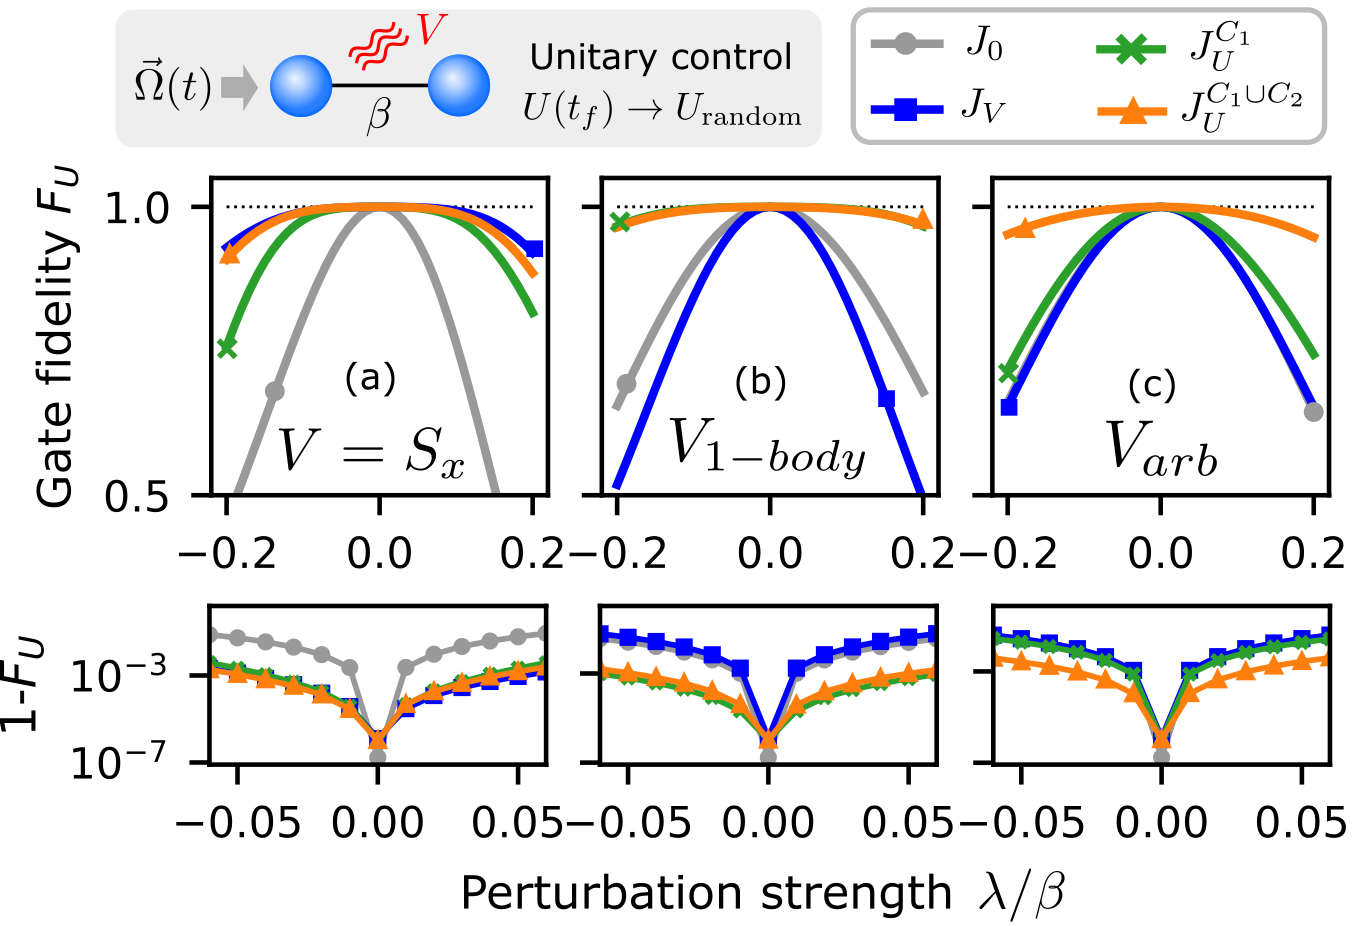
\includegraphics[
        width=\textwidth,
        height=0.63\textheight,
        keepaspectratio
      ]{figures/poggi2024_fig2.png}
    \end{column}
  \end{columns}
  \vspace{-1mm}
  \source{Poggi et al., PRL 132, 193801 (2024), Fig. 2}
\end{frame}

\begin{frame}{核心结论}
  \small
  \explain{第一步：误差被理想轨迹旋转，并在整个控制时间内平均。}
  \[
    \boxed{
    H_\lambda=H_0+\lambda V
    \quad\Longrightarrow\quad
    \Vbar
    \quad\Longrightarrow\quad
    |\Vbar)=M_0|V)
    }
  \]
  \explain{第二步：\(M_0\) 统一编码所有未知方向，\(J_{\mathrm U}\) 测量其
  traceless response。}
  \[
    \boxed{
    J_{\mathrm U}=\frac1d\|\Mtilde\|_F^2,
    \qquad
    \Mtilde=M_0(\mathbb I-\mathbb P_0)
    }
  \]
  \explain{第三步：1-design 只保留 identity，因此所有 traceless
  Hamiltonian errors 的一阶平均同时消失。}
  \[
    \boxed{
    M_0=\mathbb P_0
    \quad\Longleftrightarrow\quad
    \text{unitary 1-design}
    \quad\Longrightarrow\quad
    \Vbar=0\quad\forall\,\Tr V=0
    }
  \]
  \insight{适用范围：\(|\lambda|\ll1\) 的 systematic Hamiltonian error；
  decay 与一般 non-unitary channel 需要 Liouvillian/channel-level 推广。}
\end{frame}

\end{document}
